\documentclass[a4paper, 12pt]{article}
\usepackage{graphicx, amsmath, amssymb, parskip}
\newcommand{\unit}[1]{\ensuremath{\, \mathrm{#1}}}
\begin{document}

\title{Intro to Statics}
\author{Alexander Bailey}
\maketitle
\begin{center}
\textit{Capacity must exceed demand}
\end{center}
Statics is a subsection of mechanics that focuses on bodies that are not moving.
Hence, it is the study of bodies at rest.
Statics is largely derived from Newton's second and third laws that state:

\begin{itemize}
    \item The relation between an object's mass, its acceleration, and the applied force, is: $F=ma$
    \item Forces of action and reaction are equal in magnitude and opposite in direction between two interacting rigid bodies.
\end{itemize}

\section{Defining a Force}
A force is "the action of one body upon another". Forces are vectors, they have both a magnitude and a direction.
Alternatively, it could be described as "an interaction that, when unopposed, will cause an object to move". 
From Newton's second law $F=ma$, we can see that a force is a product of a vector (a) and a scalar (m) hence
the direction of F is dependent on the direction of the acceleration. The units are as follows:  
\begin{center}
\begin{tabular}{l|l}
    Acceleration & $m/s^2$ \\
    Mass & $kg$ \\
    Force & $N$ \\
    Force & $kg\cdot m/s^2$ \\
\end{tabular}
\end{center}
\newpage
\section{Force Systems}
Force systems are systems involving forces (wow). Force systems can be 'deterministic' meaning that the vertical and horizontal components and moments sum to zero.
They can (generally) be solved in three different ways.
Although sometimes one method will be much easier than the other. The three ways we have been taught are:

\begin{itemize}
    \item $x$ and $y$ components 
    \item sine and cosine rules
    \item rotated co-ordinate systems
\end{itemize}
The $x$ and $y$ components method simply involves splitting the forces into their $x$ and $y$ components then solving
for whatever you need. The Sine and cosine rules are:
\begin{equation*}
    a^2 = b^2 + c^2 - 2bc\cos{A} 
\end{equation*}
\begin{equation*}
    \frac{\sin{A}}{\alpha} = \frac{\sin{B}}{\beta} 
\end{equation*}

\section{Moments}
Moments are defined by: $M=Fd$.
That is they are \textit{force $\times$ perpendicular distance}
Moments are the static equivalents of torque and have the same units $Nm$.
Moments are the result of forces that turn a body, these are sometimes called \textit{actions}.
\subsection{Solving Moment Questions}
Solving Moment Questions can be as easy as three (general) steps:
\begin{enumerate}
    \item Decompose the force vectors into their x and y components 
    \item Find the distance from the reference point for each force vector
    \item For each reference point, multiply the force components by their perpendicular distance and sum them 
\end{enumerate}
\newpage
\subsection{Example}
\begin{center}
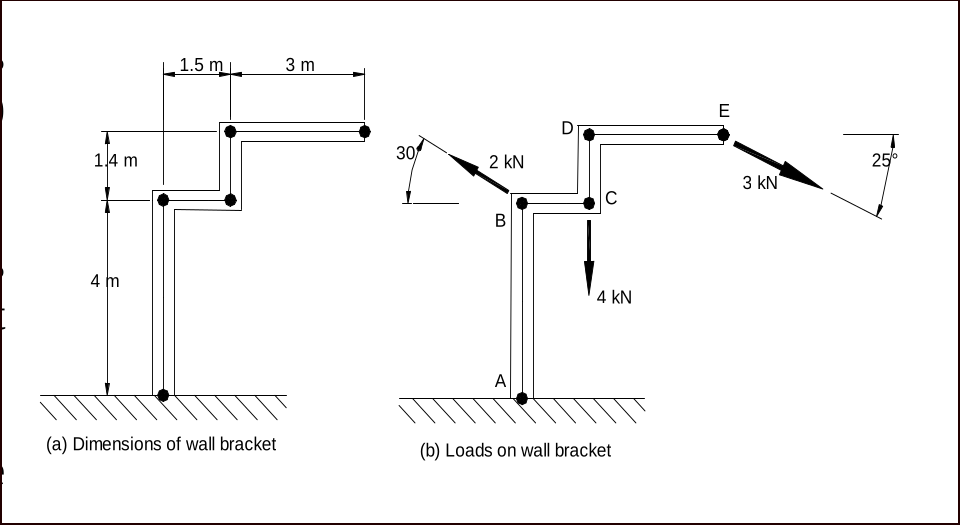
\includegraphics[scale=0.2]{topic-3}

Finding the moment around A
\end{center}
\begin{gather*}
    F_{2x} = 2\cos{30} \\ 
    F_{2y} = 2\sin{30} \\
    F_{4x} = 0 \\ 
    F_{4y} = -4 \\
    F_{3x} = 3\cos{25} \\
    F_{3y} = -3\sin{25} \\
    d_{2y} = 4m \\
    d_{2x} = 0m \\
    d_{4x} = 1.5m \\
    d_{4y} = 4m \\
    d_{3y} = 5.4m \\
    d_{3x} = 4.5m \\
    M_a = F_{2x} \cdot d_{2y} + F_{2y} \cdot d_{2x} + F_{4x} \cdot d_{4y} + F_{4y} \cdot d_{4x} + F_{3x} \cdot d_{3y} + F_{3y} \cdot d_{3x} \\
    M_a = F_{2x} \cdot d_{2y} + F_{4y} \cdot d_{4x} + F_{3x} \cdot d_{3y} + F_{3y} \cdot d_{3x} \\
    M_a = 2\cos{30} \cdot 4 + -4 \cdot 1.5 + 3\cos{25} \cdot 5.4 - 3\sin{25} \cdot 4.5 \\ 
    M_a = 19.46 \unit{kNm}
\end{gather*}
\subsection{Couples}
A couple is two forces that have equal magnitude but opposite direction, but that do not have the same line of action.
These forces sum to zero, but generate a moment. The value of a moment is simply the moments of the two forces subtracted from one another.
Or, alternatively, The magnitude of the two forces times by the distance between them.
COUPLES HAVE NEVER BEEN IN A 121 EXAM BEFORE.

\section{Resultants}
In engineering it is more common to represent a set of forces acting on an object as its \textit{resultant} instead of individual forces.
Hence you have a single vector with a magnitude and angle that could represent multiple forces acting on an object. 
The resultant is simply the sum of all the forces acting on an object (adding the $x$ and $y$ components of course). 
The difficulty with these problems comes from finding where to place the resultant on an object.
\subsection{Where to place the resultant} 
When beginning the problem, we chose a point of reference.
Sensible points of reference will be the origin or a point where a force acts.
Anywhere that you have data for will do but technically you can use any point.
You can calculate $x$ and $y$ distances for the line of action with $X=\frac{M_r}{R_y}$,$Y=\frac{M_r}{R_x}$.
This is simply a rearranging of the moments formula but let's do an example.

\begin{center}
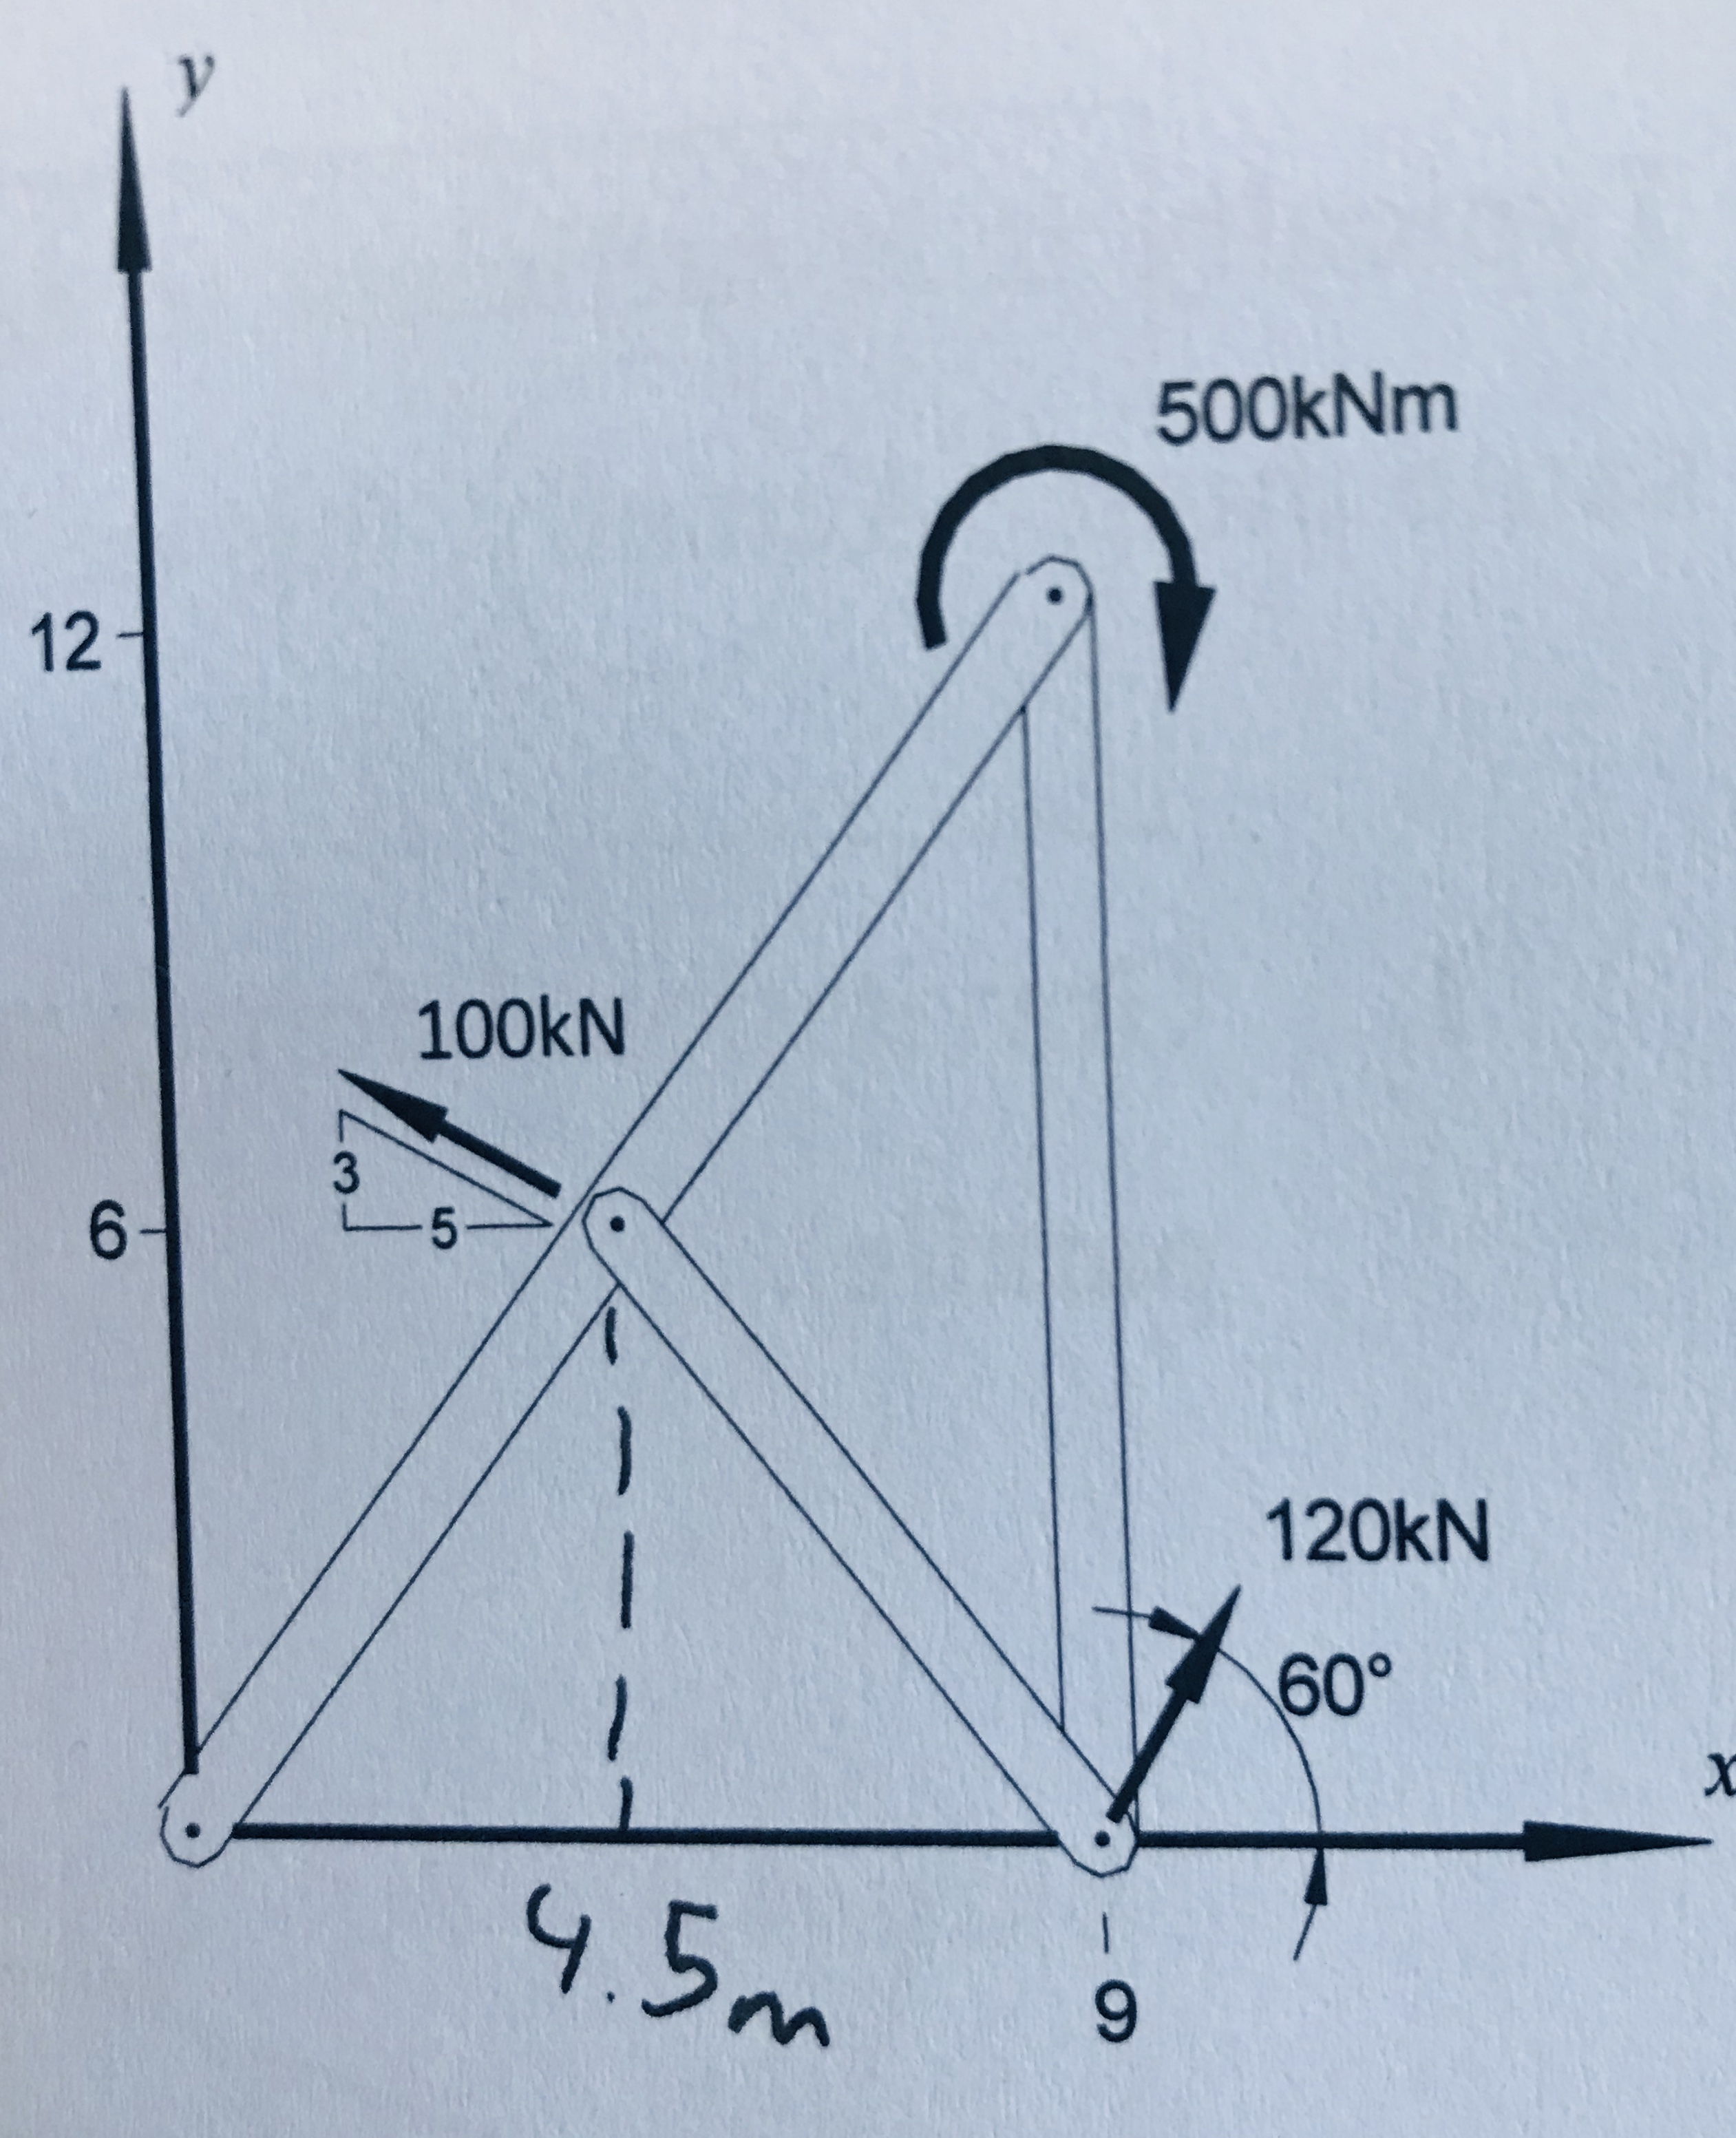
\includegraphics[scale=0.04]{4}
\begin{gather*}
    \theta = \arctan{\frac{3}{5}} = 30.96 \\
    R_x = 120\cos{60} - 100\cos{39.6} \\
    R_y = 100\sin{30.96} + 120\sin{60} \\
    |R| = \sqrt{R_x^2+R_y^2} = 157.49\unit{kN} \\
    \theta_r = \arctan{\frac{R_y}{R_x}} = 99.4 \\
    % M_o = -500 + (120\sin{60}\cdot9) + (100\sin{59.04}\cdot4.5) + (100\cos{58.04}\cdot6) \\
    M_o = 157.49\unit{kN} \\
    X = \frac{M_0}{R_y} = 7.27\unit{m} \\
    Y = \frac{M_0}{R_x} = 43.88\unit{m} \\
\end{gather*}
\end{center}
\newpage

\section{Centroids}
The centroid of a given shape is where the centre of gravity and mass act for a body of uniform thickness and density.
This is a safe assumption to make in 121 but centroids are important for other things. 
They are specific to a shape and don't take into account masses like we did in level 2/3. 
It is essentially the same calculation as CoM but using areas and in 2D. 

% \begin{equation*}
%     \bar{x} = \frac{\sum x_nA_n}{A_t} 
% \end{equation*}
% \begin{equation*}
%     \bar{y} = \frac{\sum y_nA_n}{A_t} 
% \end{equation*}
\subsection{Finding the centroid of an area}
Finding the centroid of a shape is as simple as:
\begin{itemize}
    \item Splitting the shape into smaller regular shapes (rectangles, triangles, circles)
    \item Calculating the areas and centroids of those shapes
    \item Summing these areas/centroids using the given equation for both $\bar{x}$ and $\bar{y}$
\end{itemize}

\subsection{Finding the centroid of regular shapes}
\subsubsection{Rectangles}
Rectangles are easy, just half the width or height and get your $\bar{x}$ or $\bar{y}$.
Just make sure to account for where the rectangle is placed in reference to your origin.
\subsubsection{Circles}
Circles are very similar. Half the diameter. At the centre.
\subsubsection{Triangles}
Triangles are a little harder. 
A rule you can use is:
Two thirds from the skinny end, one third from the fat end. 
This is rather  intuitive because the centroid will obviously be closer to the side with more area/mass. 
So for a triangle with a height of 4 and a width of 3 (assuming the skinny end is placed at the origin),
the centroid will be at ($\bar{x}=2,\bar{y}=\frac{4}{3}$).

\begin{center}
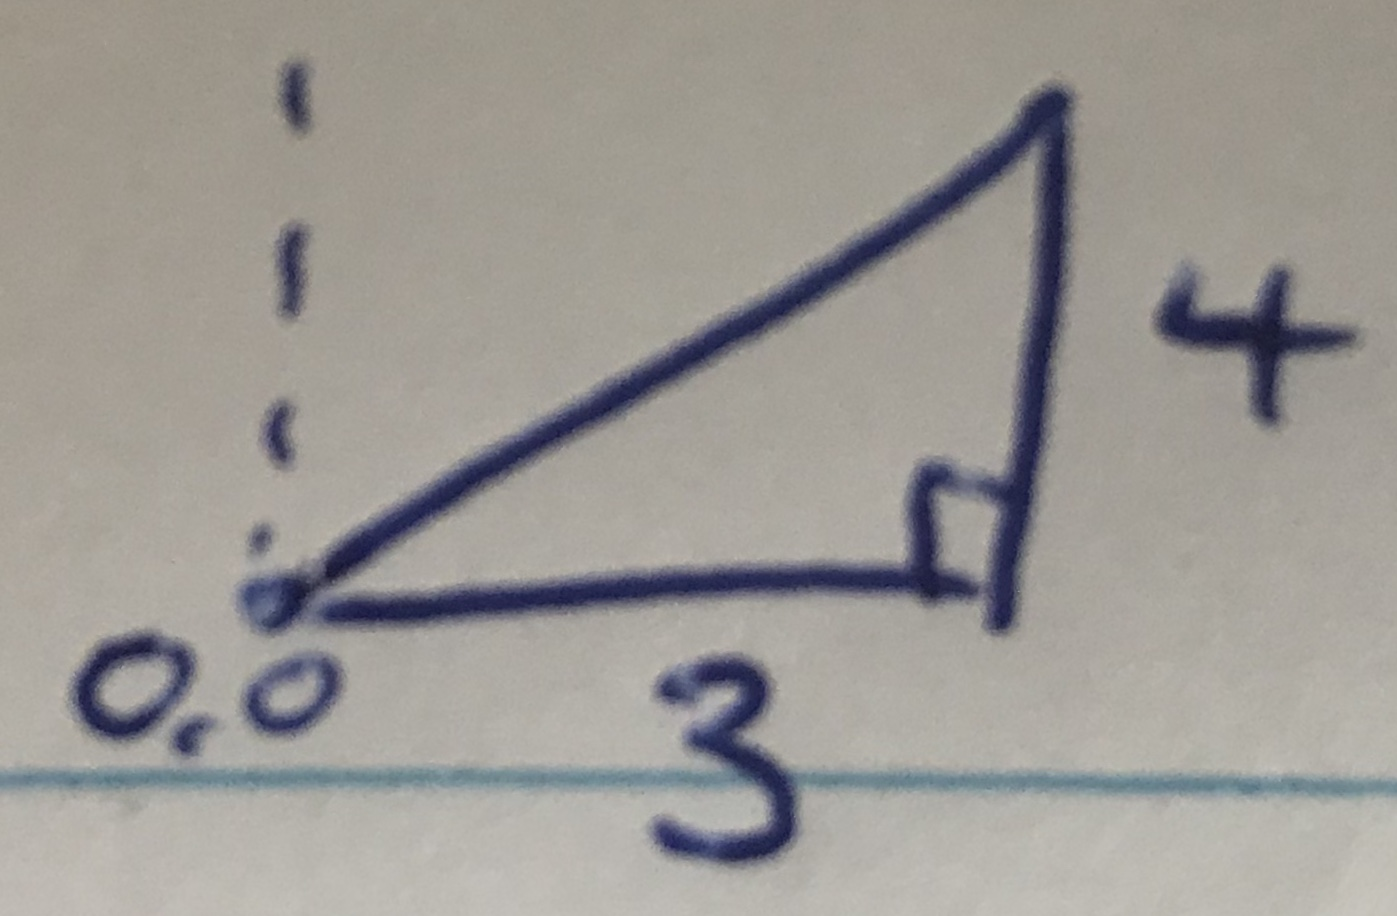
\includegraphics[scale=0.05]{triangle}
\end{center}

\subsection{Example}
\begin{center}
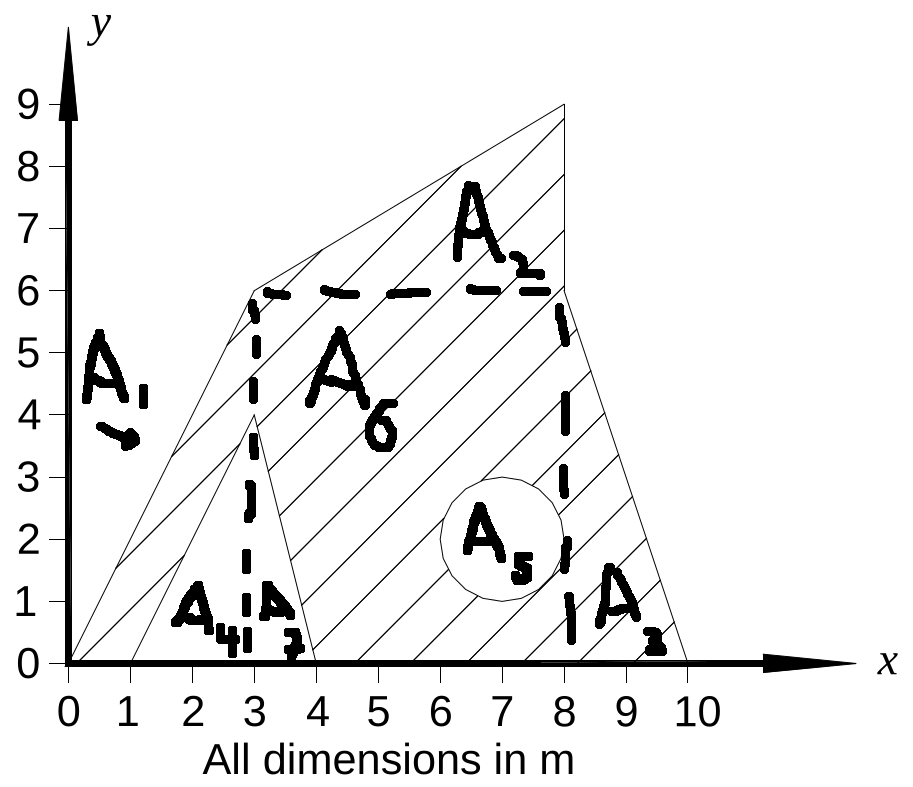
\includegraphics[scale=0.15]{centroids}
\end{center}
\begin{equation*}
\begin{gathered}
    A_1 = \frac{1}{2} \cdot 3 \cdot 6 = 9\\
    A_2 = \frac{1}{2} \cdot 5 \cdot 3 = 7.5\\
    A_3 = \frac{1}{2} \cdot 2 \cdot 6 = 6\\
    A_4 = \frac{1}{2} \cdot 1 \cdot 4 = 2\\
    A_5 = \pi \\ 
    A_6 = 30 \\ 
    A_7 = \frac{1}{2} \cdot 2 \cdot 4 = 4\\
    A_t = \sum A_n = 43.36\\ 
    \bar{x}_1 = 2 \\
    \bar{x}_2 = 6.333 \\
    \bar{x}_3 = 8.666 \\
    \bar{x}_4 = 2.333 \\
    \bar{x}_5 = 7 \\
    \bar{x}_6 = 5.5 \\
    \bar{x}_7 = 3.333 \\
    \bar{x} = \frac{\sum x_n A_n}{A_t} \\
    \bar{x} = \frac{2 \cdot 9 + 6.333 \cdot 7.5 + 8.666 \cdot 6 + 2.333 \cdot 2 + 7 \cdot \pi + 30 \cdot 5.5 + 3.333 \cdot 4}{43.36} \\
\end{gathered}
\end{equation*}

\section{Truss Problems}
Structures contain members. A member is essentially anything that makes up the structure i.e a beam or support. 
Members can contain tensions or compressions. A truss is a collection of members made using triangles. You take
three free-moving members and make a triangle and they can't move any longer. Hence, trusses. The force in a 
member is either tension (T) or compression (C) and you must mark it as such in your calculations. 
It may not be obvious which members are under which forces so we assume all members are under Tension 
(forces act away from joint) and then if they come out negative mark it as Compression. 

\subsection{Method of Joints}
The method of joints is simply solving trusses and structures by evaluating the joints between members. 
In a statics problem each joint will be in static equilibrium, hence you can solve using:
\begin{align*}
    \sum_{}F_x=0 && \sum_{}F_y=0  
\end{align*}

\subsection{Method of Sections}
Using methods of sections, you make 'cuts' in the diagram and then use moments
and forces to calculate the desired forces. At a point: $\sum_{}M=0$. The only thing is
you must ensure that when taking cuts, you cut through at least THREE members. 

The other thing is, you may want to cut through the members you are solving for. This makes 
the forces readily available to solve. Additionally, make sure you check your reactions
using $\sum F_v = 0$. 
\subsection{Example}
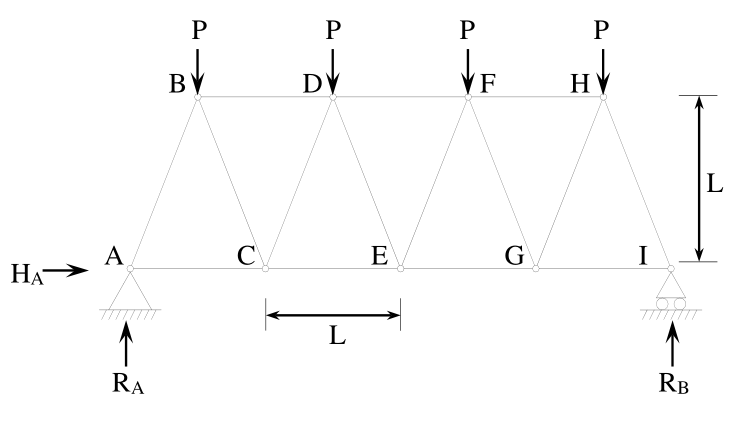
\includegraphics[scale=0.5]{truss}
\begin{align*}
    &\text{Step one for every question, DRAW THE FREEBODY DIAGRAM!} \\
    &\text{Step two, find the reactions} \\
    &R_B + R_A = 4P \\
    &R_B, R_A = 2P \\
    &H_A = 0 \\
    &\text{Step three, make a cut (don't forget to draw another FBD) and solve} \\
    &\sum M_c = 0 \\
    &\implies -2P \cdot L - L \cdot F_{BD} + \frac{1}{2}L \cdot P \\
    &F_{BD} = \frac{1.5LP}{-L} = -1.5P = 1.5P (C) \\
    &\theta = \arctan{\frac{L}{0.5L}} = 63.4^{\circ} \\
    &\sum F_v = 0 \\
    &\implies F_{CD} \cdot \sin{63.4} - P + 2P = 0 \\
    &F_{CD} = \frac{-P}{sin(63.4)} = 1.12P (C) \\
    &\sum M_D = 0 \\
    &-PL - 2P \cdot 1.5L + F_{CE} \cdot L = 0 \\
    &F_{CE} = \frac{2PL}{L} = 2P (T) \\
\end{align*}

\section{Distributed Loads}
Distributed loads are relatively easy. Almost ALL real loads are distributed but we model them as 
simple point loads, this is what you'll do for all UDLs (Uniformly Distributed Loads) in this course. 
The only thing other thing is triangular distributed loads or "linearly varying load" (LVL). We simply 
replace these with two (or more) point loads.

\subsection{Linearly Varying Loads}
LVLs (read: triangle loads) are the only slightly annoying part of distributed loads. Just remember "$\frac{1}{3}$rd from 
the fat end, $\frac{2}{3}$rds from the skinny end". The centroid is where the point mass will act. As for the magnitude 
of the force, it is just the 'height' of the force per distance times it's length when split up.

\subsection{Solving problems with distributed loads}
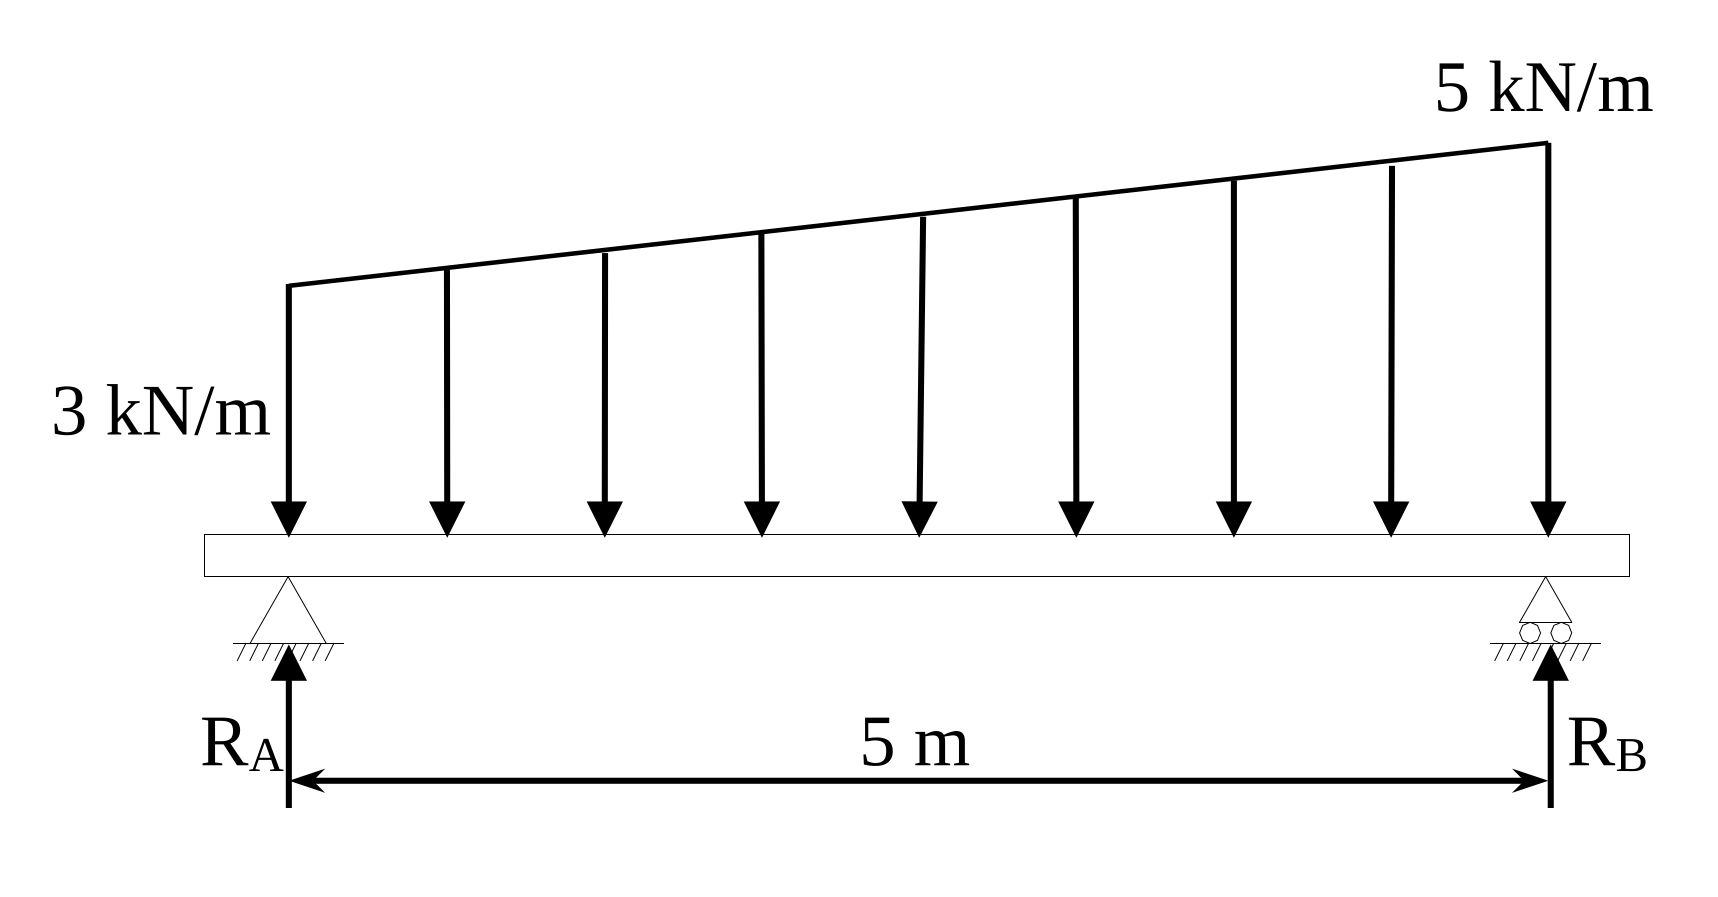
\includegraphics[scale=0.2]{lvl} \\*
Splitting the triangle into a rectangle of height 3 and a triangle of height 2 
\begin{align*}
    W_1 = 3 \text{kN/m} * 5 = 15\text{kN} \\
    \bar{x_1} = \frac{L}{2} = 2.5\text{m} \\
    W_2 = 0.5 \cdot 5 \cdot 2 = 5\text{kN} \\
    \bar{x_2} = \frac{2L}{3} = 3.33\text{m} \\
\end{align*}
Then you can use the forces to solve the rest of the problem (find $R_a$ etc)

\section{Bending and Shear}
Bending and Shear moment diagrams show the internal forces acting on a beam and are used
for structural analysis. When making a cut through a beam in a static situation, the 
internal forces must cancel the external forces. The BMD will be the integral of the SFD so
when there is a flat line (constant) in the SFD it should be a line with constant gradient in
the BMD. When there is a constant gradient line in the SFD there should be a parabola in the BMD etc.
Here we can calculate internal forces as we move the cut along the beam.

Positive bending will be like a happy face, negative bending (less commmon, also called hogging)
is like a sad face. 

\section{Friction} 
Friction is a force that opposes motion caused by the inherent imperfect roughness of two surfaces. 
The force required to cause sliding of a mass (purely horizontal motion) is dependent on F (the friction force)
where F is dependent upon N (the normal force, reaction of the support (ground)). Thus, F (the force due to friction) 
is given by $F=\mu N$ where $\mu$ is the coefficient of friction. IMPORTANT NOTE: There are two 'coefficients of friction', $\mu_k$ and $\mu_s$.
These are the coefficients of static friction and kinetic friction. Unless stated, assume: $\mu = \mu_k = \mu_s$.

$F = \mu N$ describes the magnitude only at the critical threshold just before motion 
would commence i.e the maximum friction force. Keep in mind, friction is a reaction so can only act with up to the level of the loading. 
The friction coefficient is usually stated or they might ask you to calculate it. The angle of the slop that will cause a body to slip down
a slope regardless of weight is given by: $\phi = \arctan{\mu}$. Additionally, $\phi$ is the angle of the resultant of F (friction) and N (the normal force). 

\subsection{Example}
\begin{align*}
    &W = 981N \\
    &\sum F_y = 0 \\
    &\implies N - 981\cos{20} - P\sin{20} = 0 \\
    &\implies N = 921.8 + 0.342P \\
    &\sum F_x = 0 \\
    &\implies P\cos{20} - 981\sin{20} - F = 0 \\
    &\implies F - 0.940P = -335.5 \\
    &\because F = 0.3N \\
    &\implies 0.3(921.8 + 0.342P) - 0.940P = -335.5 \\
    &\therefore P = \frac{-612.0}{-0.837} = 731N \\
\end{align*}

\section{Supports}
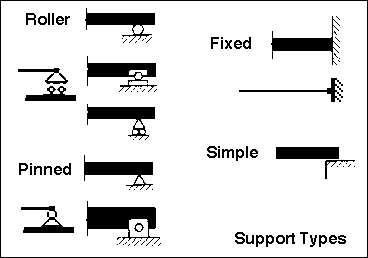
\includegraphics[scale=0.5]{supports}
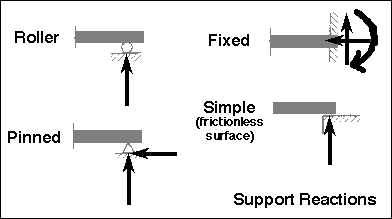
\includegraphics[scale=0.59]{supports-reactions}

\end{document}
